\documentclass[acmsmall]{acmart}
\usepackage{subcaption}
\usepackage{float}

%%
%% \BibTeX command to typeset BibTeX logo in the docs
\AtBeginDocument{%
  \providecommand\BibTeX{{%
    \normalfont B\kern-0.5em{\scshape i\kern-0.25em b}\kern-0.8em\TeX}}}

%% Rights management information.  This information is sent to you
%% when you complete the rights form.  These commands have SAMPLE
%% values in them; it is your responsibility as an author to replace
%% the commands and values with those provided to you when you
%% complete the rights form.
\setcopyright{none}
\copyrightyear{2020}
\acmYear{2020}
\renewcommand\footnotetextcopyrightpermission[1]{}
\acmDOI{}
\pagestyle{plain}
\settopmatter{printacmref=false}


%%
%% Submission ID.
%% Use this when submitting an article to a sponsored event. You'll
%% receive a unique submission ID from the organizers
%% of the event, and this ID should be used as the parameter to this command.
%%\acmSubmissionID{123-A56-BU3}

%%
%% The majority of ACM publications use numbered citations and
%% references.  The command \citestyle{authoryear} switches to the
%% "author year" style.
%%
%% If you are preparing content for an event
%% sponsored by ACM SIGGRAPH, you must use the "author year" style of
%% citations and references.
%% Uncommenting
%% the next command will enable that style.
%%\citestyle{acmauthoryear}

%%
%% end of the preamble, start of the body of the document source.
\begin{document}

%%
%% The "title" command has an optional parameter,
%% allowing the author to define a "short title" to be used in page headers.
\title{Author Attribution – DerStandard Forum Writing Style}

%%
%% The "author" command and its associated commands are used to define
%% the authors and their affiliations.
%% Of note is the shared affiliation of the first two authors, and the
%% "authornote" and "authornotemark" commands
%% used to denote shared contribution to the research.
\author{Patrick Deutschmann}
\email{patrick.deutschmann@tugraz.at}

\author{Lukas Timpl}
\email{lukas.timpl@tugraz.at}


%%
%% The abstract is a short summary of the work to be presented in the
%% article.
\begin{abstract}
  %TODO write abstract
\end{abstract}

%%
%% The code below is generated by the tool at http://dl.acm.org/ccs.cfm.
%% Please copy and paste the code instead of the example below.
%%
\begin{CCSXML}
<ccs2012>
   <concept>
       <concept_id>10010147.10010178.10010179</concept_id>
       <concept_desc>Computing methodologies~Natural language processing</concept_desc>
       <concept_significance>500</concept_significance>
       </concept>
 </ccs2012>
\end{CCSXML}

\ccsdesc[500]{Computing methodologies~Natural language processing}
%%
%% Keywords. The author(s) should pick words that accurately describe
%% the work being presented. Separate the keywords with commas.
\keywords{natural language processing, neural networks, author attribution, RNN}


%%
%% This command processes the author and affiliation and title
%% information and builds the first part of the formatted document.
\maketitle

\section{Problem Setting}
%TODO @Patrick


\section{Related Work}
%TODO @Patrick


\section{Setup}
%TODO @Patrick


\section{Features}
To best utilize our dataset we made use of various different features which are described in this section. 

\subsection{Post Metadata}
The dataset contains a number of values we consider as meta-data, data that is not directly related to the actual text of the post and can be computed without considering the actual content of the post. 

\subsubsection{Date Statistics}
For this feature we analysed at which time of the day and on which day of the week users write their posts. 
The notion behind this was, that individual users will tend to at similar times.
A histogram of this data is depicted in Figure~\ref{fig:date_stats}.

\begin{figure}[H]
\centering
\begin{subfigure}{.5\textwidth}
\centering
  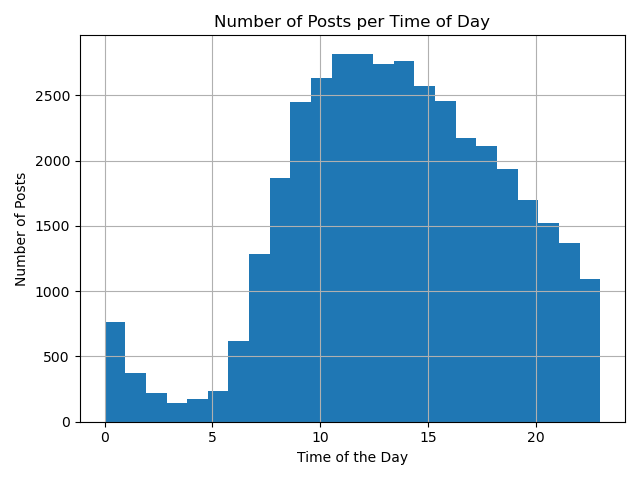
\includegraphics[width=.9\linewidth]{assets/Number_of_posts_per_time_of_day.png}
 \end{subfigure}%
\begin{subfigure}{.5\textwidth}
\centering
  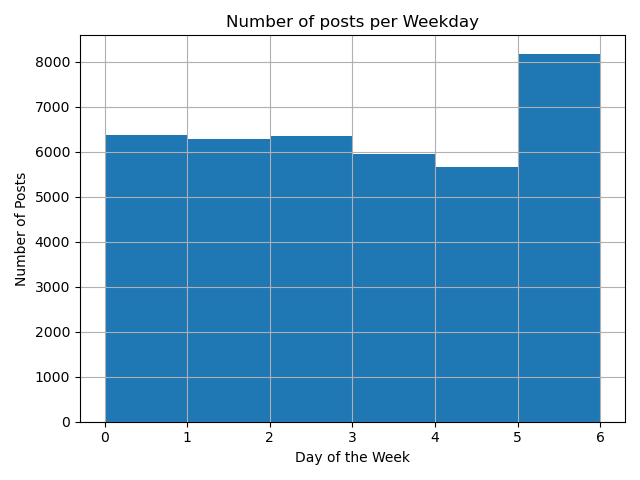
\includegraphics[width=.9\linewidth]{assets/Number_of_posts_per_day_of_week.png}
 \end{subfigure}
 \caption{Date Statistics}
\label{fig:date_stats}
\end{figure}

\subsubsection{Post Ratings and Parent Posts}
For further information about a post without the actual content we looked at the post ratings and whether the post was a comment to another users post. The aim with this feature was to identify users that post more controversial content as well as users that only ever post comments (have a parent post) and users that never answer to other users (no parent post). Again we depict a histogram over this data (Figure~\ref{fig:post_stats}). This figure clearly shows, that most posts get no votes at all, while there are a few posts which get a very large number of votes. 

\begin{figure}[H]
\centering
\begin{subfigure}{.5\textwidth}
\centering
  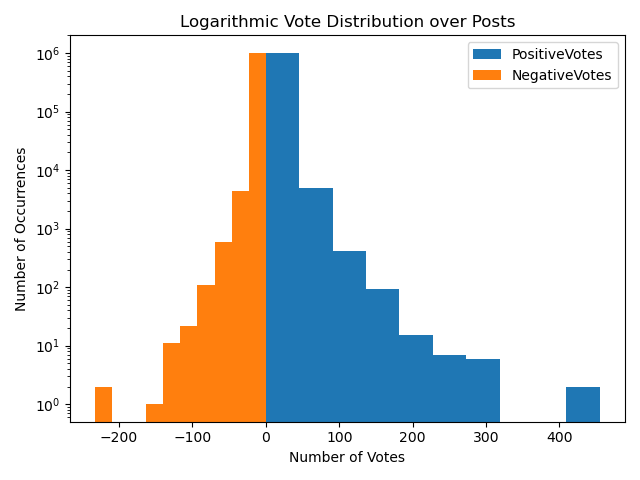
\includegraphics[width=.9\linewidth]{assets/Logarithmic_Vote_Distribution_over_Posts.png}
 \end{subfigure}%
\begin{subfigure}{.5\textwidth}
\centering
  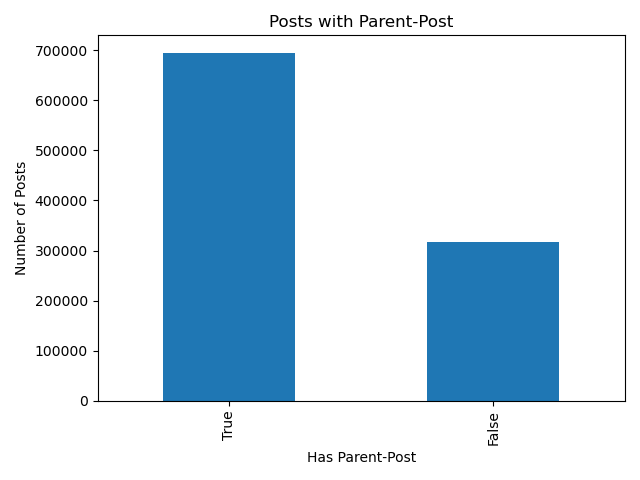
\includegraphics[width=.9\linewidth]{assets/Posts_with_parent_post.png}
 \end{subfigure}
 \caption{Post Statistics}
\label{fig:post_stats}
\end{figure}

\subsubsection{Article Categories}
Articles in the dataset also contain a path which we used as a categorical feature with the idea, that individual users will be more interested in particular topics and therefore are more likely to write post under those articles. A histogram of the number of posts in each category of the most common main category "Newsroom" is depicted in Figure~\ref{fig:article_categories}.

\begin{figure}[H]
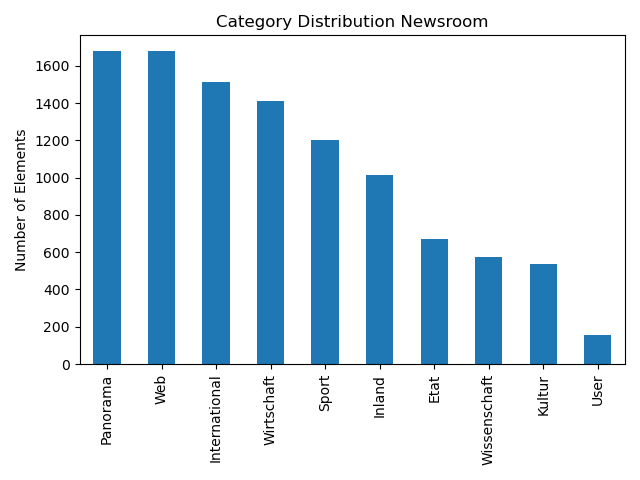
\includegraphics[width=.5\linewidth]{assets/Category_Distribution_Newsroom.png}
\caption{Article Category Distribution}
\label{fig:article_categories}
\end{figure}


\subsubsection{Article Named Entities}
To get a more detailed view of the interests of users additionally to the Article Categories, we also analysed Named Entities in the articles under which the posts where written. Similarly to the Article Categories, the notion behind this was, that individual users will be more interested in certain entities and hence are more likely to write a post under Articles containing these Entities. \\
For this we utilized the library Flair (\url{https://github.com/flairNLP/flair}) a library that offers state-of-the-art Named Entity Recognition for German language. Histograms for the recognized entities are depicted in Figure~\ref{fig:named_entities}.

\begin{figure*}[h!]
        \centering
        \begin{subfigure}[b]{0.475\textwidth}
            \centering
            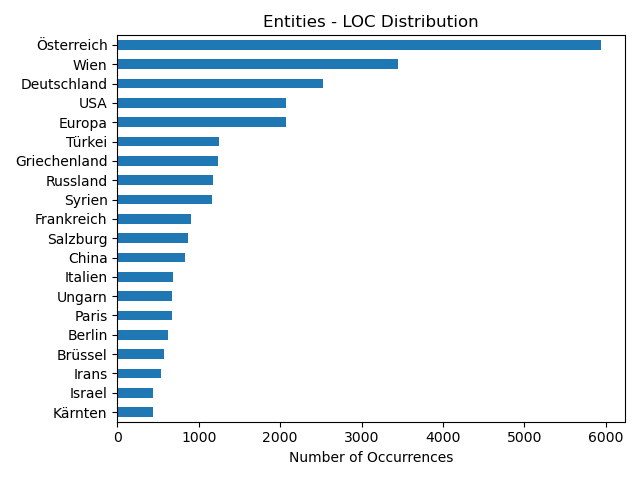
\includegraphics[width=\textwidth]{assets/Entities_LOC_Distribution.png}
        \end{subfigure}
        \begin{subfigure}[b]{0.475\textwidth}  
            \centering 
            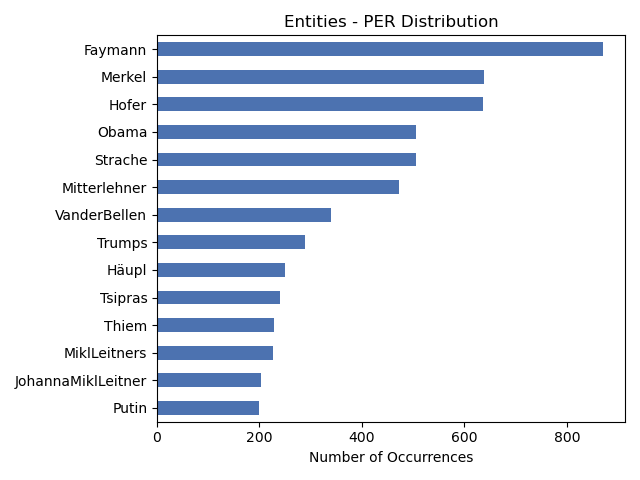
\includegraphics[width=\textwidth]{assets/Entities_PER_Distribution.png}
        \end{subfigure}
        \begin{subfigure}[b]{0.475\textwidth}   
            \centering 
            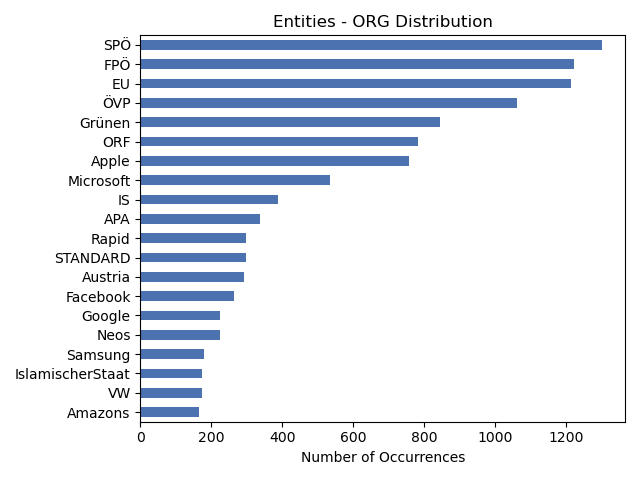
\includegraphics[width=\textwidth]{assets/Entities_ORG_Distribution.png}
        \end{subfigure}
        \begin{subfigure}[b]{0.475\textwidth}   
            \centering 
            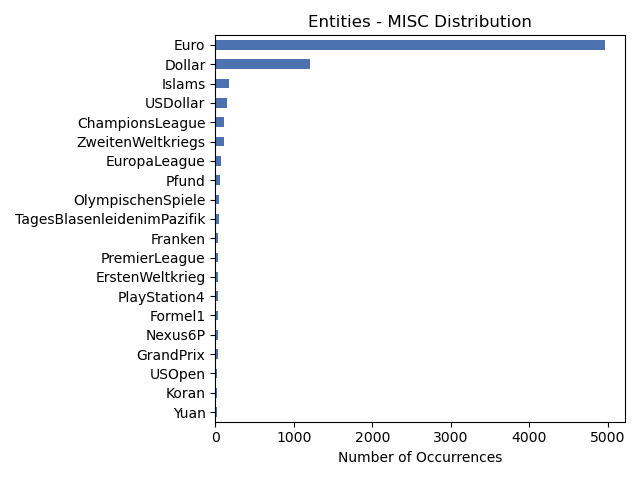
\includegraphics[width=\textwidth]{assets/Entities_MISC_Distribution.png}
        \end{subfigure}
         \caption{Top Entities in Articles for locations (LOC), persons (PER), organizations (ORG) and other Entities (MISC).}
         \label{fig:named_entities}
\end{figure*}


\subsection{Styleometric}
Next, we looked at the content of the posts and computed various stylometric features. These features are based on the writing style of the user. The list and description of these features can be found in Table~\ref{tab:stylometric}. We computed all of those features twice. Once for the headline of the post and once for the actual text. The notion behind this is, that we noticed, that the way in which the headline was used differed significantly between users. While some users choose to leave the field empty, some showed a clear tendency towards upper-case characters, and some wrote the headline as the start for the main text and concluded it with "...". 

\begin{table}[H]
\begin{tabular}{ll}
Feature Name & Description \\ \hline
Alpha-chars-ratio & The fraction of total characters in the paragraph which are letters \\
Digit-chars-ratio & The fraction of total characters in the paragraph which are digits \\
Upper-chars-ratio & The fraction of total characters in the paragraph which are upper-case \\
White-chars-ratio & The fraction of total characters in the paragraph which are whitespaces \\
Emoticon-chars-ratio & The number of Emoticons (e.g. ":)", ":D", ...) per total characters \\
Average-word-length & Average length of words in characters \\
Average-sentencechar-length & Average length of sentences in characters \\
Average-sentenceword-length & Average length of sentences in words \\
Total length & The length of the text \\
\end{tabular}
\caption{Used Stylometric Features}
\label{tab:stylometric}
\end{table}

\subsection{Post Embeddings}
As a final feature, we computed word embeddings for the post texts. The goal of this feature is to get information on the actual content the users write about as well as potentially additional information on their writing style. \\
To compute the vectors, we utilized the Word2Vec model of the library Gensim (\url{https://radimrehurek.com/gensim/}). 
We used embedding vectors of size 50 only computed the embedding for words which at least occurred ten times and trained the model over 500 iterations. 
When embedding the posts, we only embedded at most 100 words for each post to restrict the size of the feature.  

\section{Evaluation}
%TODO @Lukas

\subsection{Baseline}

\subsection{Results}

\subsection{Interpretation}


\section{Discussion}
%TODO

\section{Conclusion}
%TODO


%%
%% The next two lines define the bibliography style to be used, and
%% the bibliography file.
\bibliographystyle{ACM-Reference-Format}
\bibliography{sample-base}


\end{document}
\endinput

